
%
% introduction.tex
% Copyright (C) 1995 by John Heidemann, <johnh@isi.edu>.
% $Id: demo2intr.tex,v 1.1 1996/01/12 18:13:58 johnh Exp $
%

\chapter{Introduction}

In classical probability, in the context of a probability space $(\Omega,\mc{F},\mathbb{P})$ a random variable is a measurable function $X\colon \Omega\to \R$ and the \emph{moments} of a random variable are the quantities
	\begin{align*}
		E(X^n):=\int_\Omega X(\omega)^n d\mathbb{P}(\omega)\qquad n\geq 0,
	\end{align*}
which capture a great deal of information about the random variable. A random variable $X$ is often studied via its \emph{law}, which is a measure $\mu_X$ on $\R$ that completely characterizes $X$. In particular,
	\begin{align*}
		\mathbb{P}(a\leq X\leq b) = \mu_X([a,b])\qquad \forall -\infty<a\leq b<\infty,
	\end{align*}
and the law describes the moments of $X$:
	\begin{align*}
		E(X^n) = \int_\R t^n\ d\mu_X(t) \qquad \forall n\geq 0.
	\end{align*}
When considering several random variables $X_1,\ldots, X_n\colon \Omega\to \R$, their \emph{joint law} is a measure $\mu_{(X_1,\ldots, X_n)}$ on $\R^n$ satisfying
	\begin{align*}
		\mathbb{P}(X_i\in [a_i,b_i]\colon i\in\{1,\ldots,n\}) = \mu_{(X_1,\ldots, X_n)}( [a_1,b_1]\times\cdots \times [a_n,b_n]),
	\end{align*}
and for any polynomial $p\in \C[t_1,\ldots, t_n]$
	\begin{align*}
		\int_{\Omega^n} p(X_1(\omega_1),\ldots, X_n(\omega_n))\ d\mathbb{P}(\omega_1)\cdots d\mathbb{P}(\omega_n) = \int_{\R^n} p(t_1,\ldots, t_n) d\mu_{(X_1,\ldots, X_n)}(t_1,\ldots, t_n).
	\end{align*}
	
In free probability (or non-commutative probability), the context is usually a unital algebra $A$ and a positive linear functional $\phi\colon A\to \C$ satisfying $\phi(1)=1$. The elements $a\in A$ are thought of as \emph{non-commutative random variables}, and evaluation in $\phi$ corresponds to integration against $d\mathbb{P}$ in classical probability in the sense that the moments of $a$ are given by $\phi(a^n)$, $n\geq 0$. In fact, if $a=a^*$ is self-adjoint then there exists a measure $\mu_a$ on $\R$ which describes the moments of $a$:
	\begin{align*}
		\phi(a^n) = \int_\R t^n\ d\mu_a(t)\qquad \forall n\geq 0.
	\end{align*}
Thus the measure $\mu_a$ is thought of as the law of $a$.

However, if $a$ is not self-adjoint its moments are no longer necessarily described by a measure. In this case the \emph{law} of a general non-commutative random variable refers to the collection of its moments $\{\phi(a^n)\}_{n\geq 0}$. More precisely, it is a linear functional $\phi_a$ on complex polynomials on an abstract indeterminate $t$. For $p\in \C[t]$, if we write $p(a)$ for the polynomial evaluated at $t=a$ then $\phi_a$ is defined by
	\begin{align*}
		\phi_a(p):=\phi(p(a))\qquad \forall p\in \C[t].
	\end{align*}
	
More generally, the \emph{joint law} of an $n$-tuple of non-commutative random variables $(a_1,\ldots, a_n)$ in  $A^n$ is a linear functional $\phi_{(a_1,\ldots, a_n)}$ on non-commutative polynomials in abstract non-commutating indeterminates $t_1,\ldots, t_n$. For $p\in \C\<t_1,\ldots, t_n\>$, if we write $p(a_1,\ldots, a_n)$ for the polynomial evaluated at $t_1=a_1,\ldots, t_n=a_n$ then $\phi_{(a_1,\ldots, a_n)}$ is defined by
	\begin{align*}
		\phi_{(a_1,\ldots, a_n)}(p)=\phi( p(a_1,\ldots, a_n))\qquad p\in \C\<t_1,\ldots, t_n\>.
	\end{align*}

It is often the case that the $*$-algebra is either a $C^*$-algebra or a von Neumann algebra, in which case $(A,\phi)$ has additional structure. For example, if $A=M$ is a $\mathrm{II}_1$ factor, then $\phi$ is usually taken to be the unique tracial state $\tau$ on $M$. In this work, however, we shall consider non-tracial von Neumann algebras equipped with a faithful, normal, non-tracial state.

Transport, in classical probability, refers to a map $T\colon \Omega_1\to \Omega_2$ between two probability spaces $(\Omega_i,\mc{F}_i,\mathbb{P}_i)$, $i\in\{1,2\}$, such that
	\begin{align*}
		\mathbb{P}_1(T^{-1}(S))=\mathbb{P}_2(S)\qquad \forall S\in\mc{F}_2;
	\end{align*}
that is, $T_*\mathbb{P}_1=\mathbb{P}_2$. In particular, $T$ induces a measure preserving map via precomposition:
	\begin{align*}
		L^\infty(\Omega_2,\mathbb{P}_2)\ni f\mapsto f\circ T\in L^\infty(\Omega_1,\mathbb{P}_1).
	\end{align*}
Moreover, if $X_1,\ldots, X_n$ are random variables on $\Omega_2$ with joint law $\mu_{(X_1,\ldots, X_n)}$, then $X_1\circ T,\ldots, X_n\circ T$ are random variables on $\Omega_1$ with the same joint law. In this case we describe $T$ as transport from $\mu_{(X_1,\ldots, X_n)}$ to $\mu_{(X_1\circ T,\ldots, X_n\circ T)}$.

Free transport is the analogue of this latter notion. Let $(\mc{M},\theta)$ and $(\mc{N},\psi)$ be two von Neumann algebra probability spaces with faithful normal states, and let $X:=(X_1,\ldots, X_n)\in \mc{M}^n$ and $Z:=(Z_1,\ldots, Z_n)\in \mc{N}^n$ be two $n$-tuples of non-commutative random variables with joint laws $\theta_X$ and $\psi_Z$, respectively. Then transport from $\theta_X$ to $\psi_Z$  is an $n$-tuple $Y=(Y_1,\ldots, Y_n) \in W^*(X_1,\ldots, X_n)^n$ whose joint law with with respect $\theta$, say $\theta_Y$, is the same as $\psi_Z$:
	\begin{align*}
		\theta_Y(p) = \psi_Z(p)\qquad \forall p\in \C\<t_1,\ldots, t_n\>.
	\end{align*}
In particular, the densely defined map
	\begin{align*}
		W^*(Z_1,\ldots, Z_n)\ni p(Z_1,\ldots, Z_n) \mapsto p(Y_1,\ldots, Y_n)\in W^*(X_1,\ldots, X_n)\qquad p\in \C\<t_1,\ldots, t_n\>,
	\end{align*}
extends to a state-preserving embedding $W^*(Z_1,\ldots, Z_n)\hookrightarrow W^*(X_1,\ldots, X_n)$.

Transport maps are abundant in classical probability because of Brenier's monotone transport theorem \cite{Bre91}: if the joint law of classical random variables $X_1,\ldots, X_n$ is the standard Gaussian distribution on $\R^n$:
	\begin{align*}
		\frac{d\mu_{(X_1,\ldots, X_n)}}{dm_n}(t_1,\ldots, t_n) =\frac{1}{\sqrt{(2\pi)^n}} \text{exp}\left(-\frac{1}{2}\sum_{j=1}^n t_j^2\right)
	\end{align*}
(here $m_n$ is the Lebesgue measure on $\R^n$), then there exists transport from $\mu_{(X_1,\ldots, X_n)}$ to any other joint law $\mu_{(Z_1,\ldots, Z_N)}$ satisfying some technical conditions (Lebesgue absolutely continuous, finite second moment, etc.). Moreover, the transport map $T$ can be taken to be monotone: $T=\nabla G$ for some convex function $G$. In free probability, transport is much harder to come by.

In \cite{GS14}, by solving a free analogue of the Monge-Amp\'{e}re equation, Guionnet and Shlyakhtenko obtained transport from the joint law of free semi-circular random variables $X_1,\ldots, X_n \in M_{s.a.}$ in a tracial von Neumann algebra $(M,\tau)$ to certain perturbations of this joint law, which we will discuss below. A semi-circular random variable $X\in M$ is an element whose distribution with respect to $\tau$, $\tau_X$, satisfies
	\begin{align*}
		\frac{d\tau_X}{d t}(t) = \chi_{[-2,2]}(t) \frac{1}{2\pi} \sqrt{4 - t^2}.
	\end{align*}
Free semi-circular variables are the non-commutative analogue of independent Gaussian random variables, insomuch as Voiculescu's free central limit theorem (\emph{cf.} \cite{Voi91}) is precisely the classical central limit theorem with independence and Gaussian random variables replaced by free independence and semi-circular random variables, respectively. Hence this result of Guionnet and Shlyakhtenko can be viewed as a non-commutative analogue of Brenier's monotone transport theorem. Furthermore, if sufficient control on the transport variables is maintained then the state-preserving embedding guaranteed by free transport is in fact a state-preserving $*$-isomorphism. Consequently, this result provided criterion for when an $n$-tuple of non-commutative random variables generate the free group factor $L \mathbb{F}_n = W^*(X_1,\ldots, X_n)$.

The non-commutative joint laws to which Guionnet and Shlyakhtenko obtained transport to were perturbations of $\tau_{(X_1,\ldots, X_n)}$ in the following sense. The trace $\tau$ satisfies a ``free Gibbs state'' condition with respect to a ``Gaussian potential'' $V_0=\frac{1}{2}\sum X_j^2$:
	\begin{align*}
		\tau( \D(V_0) \cdot P) = \tau\otimes\tau^{op}(\J P)\qquad P\in \C\<X_1,\ldots, X_n\>^n,
	\end{align*}
where $\D$ and $\J$ are non-commutative differential operators (\emph{cf.} subsection \ref{tensor_product_notation}). Suppose $Z_1,\ldots, Z_n$ are self-adjoint elements from another tracial von Neumann algebra $(\tilde{M}, \tilde{\tau})$ whose joint law satisfies this free Gibbs state condition for some other potential $V\in W^*(Z_1,\ldots, Z_n)$. Guionnet and Shlyakhtenko showed in \cite{GS14} that provided $V$ is a convergent power series in $Z_1,\ldots, Z_n$ which is close in some Banach norm (\emph{cf.} subsection \ref{setup}) to $V_0$ (when considering both as formal power series) then transport from $\tau_{(X_1,\ldots, X_n)}$ to $\tilde{\tau}_{(Z_1,\ldots, Z_n)}$ exists. Moreover, by requiring $V$ to be closer to $V_0$ if necessary, it follows that $W^*(X_1,\ldots, X_n)\cong W^*(Z_1,\ldots, Z_n)$.
 
In the commutative case (i.e. $n=1$), the free Gibbs state condition amounts to saying that if $\eta$ is the semi-circle law ($\frac{d\eta}{dt}(t)=\chi_{[-2,2]}(t) \frac{1}{2\pi}\sqrt{4-t^2}$) and $V(t)=\frac{1}{2} t^2 + W(t)$ for $W$ analytic on a disk of radius $R$ and small $\|\cdot\|_\infty$-norm then
	\begin{align*}
		\int_\R V'(t) f(t)\ d\eta(t) = \int_\R \int_\R \frac{f(s) - f(t)}{s-t} d\eta(s) d\eta(t)
	\end{align*}
for all $f$ which are analytic on the disk of radius $R$. In general, a measure satisfying this equation is called a Gibbs state with potential $V$.

Given a potential $V$ close to $V_0$ and starting with the non-commutative free Gibbs state condition, Guionnet and Shlyakhtenko produced an equivalent condition which is amenable to a fixed point argument. Using this latter condition they show the existence of $Y_1,\ldots, Y_n$ power series in the $X_1,\ldots, X_n$ whose joint law with respect to $\tau$ satisfies the free Gibbs state condition with potential $V$. Then a result of Guionnet and Maurel-Segala in \cite{GM06} implies that this condition is uniquely satisfied by a joint law (again provided $V$ and $V_0$ are sufficiently close). Hence $Y_1,\ldots, Y_n$ serve as transport variables for any other $n$-tuple $(Z_1,\ldots, Z_n)$ whose joint law satisfies the free Gibbs condition with potential $V$.

In Chapter \ref{non-tracial transport chapter} we adapt the transport result of Guionnet and Shlyakhtenko to the context of a von Neumann algebra $M$ with a (not necessarily tracial) state $\varphi$ on $M$. The random variables $X_1,\ldots, X_N$ are no longer assumed to be free; instead their joint law is assumed to be a free quasi-free state and they generate the free Araki-Woods factor $\Gamma(\H_\R, U_t)''$ (\emph{cf.} \cite{Shl97}). While the state is no longer tracial, in this case there at least exists a positive matrix $A\in M_N(\C)$ such that
	\begin{align*}
		\varphi(X_jX_k) = \varphi\left(X_k \sum_{\ell = 1}^N [A]_{j\ell} X_\ell\right).
	\end{align*}
Really, $A$ here is encoding the action of the modular operator $\Delta_\varphi$ arising from the Tomita-Takesaki theory for $\varphi$. The Gaussian potential $V_0$ is replaced by
	\begin{align*}
		V_0:= \frac{1}{2} \sum_{j,k=1}^n \left[\frac{1+A}{2}\right]_{jk} X_k X_j.
	\end{align*}
Using the same strategy as in \cite{GS14} and making non-tracial adaptations along the way, we construct for potentials $V$ close to $V_0$ transport variables $Y_1,\ldots, Y_N$ for any other joint law which is the free Gibbs state with potential $V$. This produces a criterion for when an $N$-tuple of non-commutative random variables generate the free Araki-Woods factor $\Gamma(\H_\R,U_t)''$.


In Chapter \ref{application} we consider our first application of non-tracial free transport. Hiai developed in \cite{Hia03} a generalization of Shlyakhtenko's algebras $\Gamma(\H_\R, U_t)$ from \cite{Shl97}, called $q$-deformed Araki-Woods algebras. Letting $A$ be the generator of the one-parameter family of unitary operators $U_t=A^{it}$ $t\in \R$, Hiai was able to show the von Neumann algebras $\Gamma_q(\H_\R,U_t)''$ are factors and produced a type classification, but only in the case that $A$ has either infinitely many mutually orthogonal eigenvectors or none at all. In particular, when the Hilbert space $\H_\R$ is finite dimensional the questions of factoriality and type classification remained unanswered. An application of our result in Section \ref{application} yields $\Gamma_q(\H_\R,U_t)''\cong \Gamma(\H_\R,U_t)''$ for small $|q|$, and hence we are able to settle these questions using Theorem 6.1 in \cite{Shl97}.



In Chapter \ref{planar_algebras_chapter} we consider our second application of non-tracial free transport. Despite the relatively innocuous definition of a subfactor, Jones showed in \cite{Jon83}, \cite{Jon99}, and \cite{Jon00} that there is in fact an incredibly rich structure underlying the inclusion of one $\II_1$ factor in another. Suppose $1_B\in A\subset B$ is an inclusion of $\II_1$ factors with trace $\Tr_B$ on $B$ and trace $\Tr_A=\Tr_B\mid_A$ on $A$. Letting $e_A$ be the orthogonal projection of $L^2(B,\Tr_B)$ onto $L^2(A,\Tr_A)$, we can consider the von Neumann algebra $\<B,e_A\>\subset \B(L^2(B,\Tr_B))$ generated by $B$ and $e_A$. If the index of $A$ inside $B$
	\begin{align*}
		[B\colon A]:=\dim_A L^2(B,\Tr_B)
	\end{align*}
is finite, then $\<B,e_A\>$ is also a $\II_1$ factor with trace $\Tr_{\<B,e_A\>}$ that restricts to $\Tr_B$ on $B$. Moreover, we have $[\<B,e_A\>\colon B]=[B\colon A]$. The von Neumann algebra $\<B,e_A\>$ is called the basic construction for $A$ and $B$. Clearly this process may be iterated and doing so yields the Jones tower:
	\begin{align*}
		A_0 \subset A_1 \subset_{e_1} A_2 \subset_{e_2} A_3 \subset_{e_3} \cdots
	\end{align*}
where $A_0=A$, $A_1=B$, and $e_1=e_A$. The standard invariant of $A\subset B$ is then the lattice of higher relative commutants:
	\[
	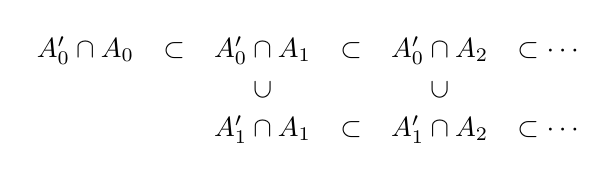
\begin{tikzpicture}[thick, scale=.5]
	\node at (0,0) {$A_0'\cap A_0$};
	
	\node at (2.25,0) {$\subset$};
	
	\node at (4.5, 0) {$A_0'\cap A_1$};
	\node at (4.5,-1) {\rotatebox{90}{$\subset$}};
	\node at (4.5,-2) {$A_1'\cap A_1$};
	
	\node at (6.75,0) {$\subset$};
	\node at (6.75,-2) {$\subset$};
	
	\node at (9,0) {$A_0'\cap A_2$};
	\node at (9,-1) {\rotatebox{90}{$\subset$}};
	\node at (9,-2) {$A_1'\cap A_2$};
	
	\node at (11.75,0) {$\subset\cdots $};
	\node at (11.75,-2) {$\subset\cdots $};
	
	\end{tikzpicture}
	\]
By studying $\lambda$-lattices, Popa found necessary and sufficient conditions for when such lattices are the standard invariant of a $\II_1$-subfactor $A\subset B$, and for each such lattice provided a construction of a canonical subfactor whose standard invariant recovered the lattice (\emph{cf.} \cite{Pop93}, \cite{Pop95}, and \cite{Pop02}).

Collecting these relative commutants as $\mc{P}:=\{\mc{P}_{n,\pm}\}_{n\geq 0}$, where for each $n\geq 0$
	\begin{align*}
		\mc{P}_{n,+}&:= A_0'\cap A_n\\
		\mc{P}_{n,-}&:= A_1' \cap A_{n+1},
	\end{align*}
defines a subfactor planar algebra. More generally, a planar algebra is a collection of graded vector spaces $\{P_{n,\pm}\}_{n\geq 0}$ which admits an action by planar tangles: diagrams which encode multilinear maps. A subfactor planar algebra is a planar algebra which satisfies some additional analytic properties.

In \cite{GJS10} Guionnet, Jones, and Shlyakhtenko use free probabilistic methods to construct a subfactor with $\mc{P}$ as its standard invariant, and hence is an alternative approach to Popa's earlier result. Given a subfactor planar algebra $\mc{P}$, for each $k\geq 0$ one can turn $Gr_k^+\mc{P}=\oplus_{n\geq k} \mc{P}_{n,+}$ into a $*$-algebra with a trace $Tr_{k,+}$ defined by a particular pairing with Temperley-Lieb diagrams.  Then each $Gr_k^+\mc{P}$ embeds into the bounded operators on a Hilbert space and generates a $\text{II}_1$ factor $M_{k,+}$. Moreover, one can define inclusion maps $i^{k-1}_k\colon M_{k-1,+}\to M_{k,+}$ so that the standard invariant associated to the subfactor inclusion $i_k^{k-1}(M_{k-1,+})\subset M_{k,+}$ (for any $k\geq 1$) recovers $\mc{P}$. The embedding relies on the fact that a subfactor planar algebra $\mc{P}$ always embeds into the planar algebra of a bipartite graph $\mc{P}^\Gamma$ (\emph{cf.} \cite{Jon00}, \cite{JP11}, and \cite{MW10}). 

It turns out that $Gr_0^+\mc{P}$ embeds as a subalgebra of a free Araki-Woods factor. In Chapter \ref{planar_algebras_chapter} we show that the free transport machinery can be encoded via planar tangles and provide an application of free transport to finite depth subfactor planar algebras.

Let $\mc{P}$ be a finite depth subfactor planar algebra and $Tr\colon \mc{P}\to\C$ be the state induced by the Temperley-Lieb diagrams via duality. By using the transport construction methods of Chapter \ref{non-tracial transport chapter}, we show that we can perturb the embedding constructed in \cite{GJS10} to make it state-preserving for states on $\mc{P}$ which are ``close'' to $Tr$. Moreover, the von Neumann algebra generated by the subfactor planar algebra via this embedding is unchanged. In this context, if $\mc{P}$ embeds into $\mc{P}^\Gamma$ and $\mu$ is the Perron-Frobenius eigenvector for the bipartite graph $\Gamma$, then the generator $A$ associated to the free Araki-Woods factor will be determined by $\mu$.

The free transport methods in \cite{GS14} and Chapter \ref{non-tracial transport chapter} apply only to joint laws of finitely many non-commutative random variables. Since each edge in the graph $\Gamma$ will correspond to a non-commutative random variable, we can only consider finite depth subfactor planar algebras with these methods.
